\documentclass{article}
\usepackage{graphicx}
\usepackage[a4paper, margin=2.5cm, top=1cm]{geometry}
\usepackage[ngerman]{babel}
\usepackage[utf8]{inputenc}
\usepackage[T1]{fontenc}

\setcounter{secnumdepth}{0}
\setlength{\parindent}{0pt}

\title{\textbf{Die Vier Seiten einer Nachricht}\\nach Schulz von Thun}
\author{Martin Kistler}
\date{April 2025}

\begin{document}

\maketitle
\thispagestyle{empty}
Schulz von Thun geht davon aus, dass jede Nachricht, die wir äußern, vier Botschaften gleichzeitig enthält – unabhängig davon, ob wir uns dessen bewusst sind oder nicht. Diese vier Seiten sind:

\subsection{1. Sachseite}
\textbf{Worüber ich informiere} – Die sachliche Information, die in der Nachricht steckt.

\vspace{0.2cm}
Beispiel: \textit{„Die Ampel ist grün.“}  

\subsection{2. Selbstoffenbarungsseite}
\textbf{Was ich von mir selbst preisgebe} – Hinweise auf Gefühle, Werte, Absichten oder persönliche Einstellungen des Senders.

\vspace{0.2cm}
Beispiel: \textit{„Ich habe es eilig.“}

\subsection{3. Beziehungsseite}
\textbf{Was ich von dir halte und wie ich zu dir stehe} – Die Art und Weise, wie die Beziehung zwischen Sender und Empfänger mitschwingt.

\vspace{0.2cm}
Beispiel: \textit{„Ich vertraue deinen Fahrkünsten nicht.“}

\subsection{4. Appellseite}
\textbf{Wozu ich dich veranlassen möchte} – Was ich beim Empfänger erreichen will, sei es bewusst oder unbewusst.

\vspace{0.2cm}
Beispiel: \textit{„Fahr schneller!“}

\section{Die Empfangsseite}
Auch der Empfänger hört auf vier Ebenen gleichzeitig – je nachdem, welche Seite er besonders betont, kann es zu Missverständnissen kommen. Ein harmloser Sachhinweis kann z.B. als Kritik (Beziehungsseite) verstanden werden. Kommunikation gelingt nur, wenn Sender und Empfänger sich über alle vier Ebenen bewusst sind.

\vspace{1cm}
\begin{figure}[h]
    \centering
    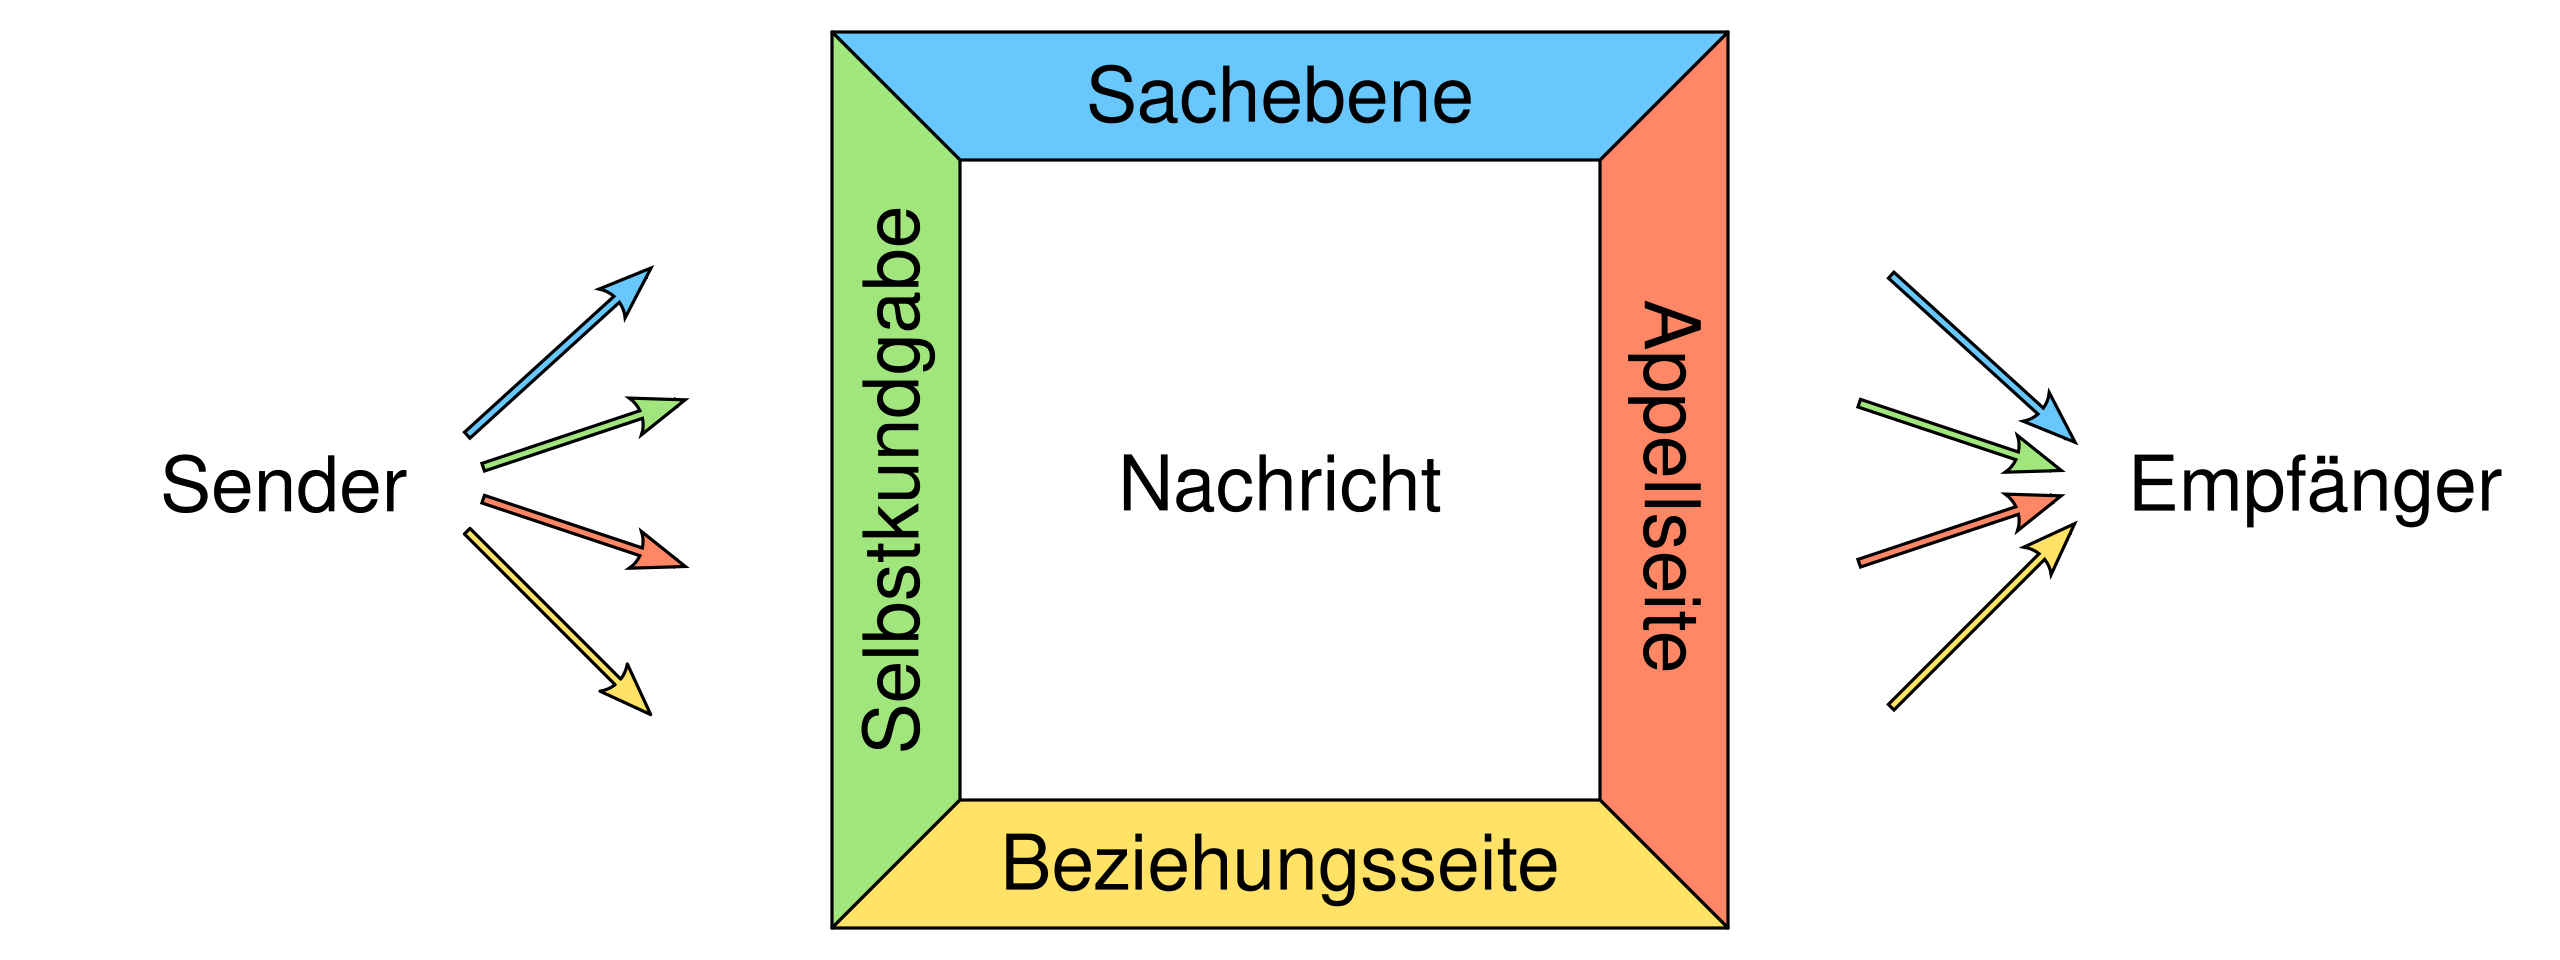
\includegraphics[width=0.25\linewidth]{nachrichtenquadrat.png}
    \caption{Das Nachrichtenquadrat}
    \label{fig:Nachrichtenquadrat}
\end{figure}

\end{document}
